\documentclass[11pt,a4paper]{article}

% Packages
\usepackage[margin=2.5cm]{geometry}
\usepackage[expansion=false]{microtype}
\usepackage{graphicx}
\usepackage{tikz}
\usetikzlibrary{shapes,arrows.meta,positioning,calc,fit,backgrounds,shadows.blur,decorations.pathmorphing,decorations.pathreplacing}
\usepackage{colortbl}
\usepackage{enumitem}
\usepackage{booktabs}
\usepackage{longtable}
\usepackage{hyperref}
\usepackage{xcolor}
\usepackage{fancyhdr}
\usepackage{titlesec}
\usepackage[most]{tcolorbox}
\usepackage{multicol}
\usepackage{amsmath,amssymb}
\usepackage{multirow}
\usepackage{setspace}
\usepackage{fontawesome5}
\usepackage{listings}

% Spacing
\setlength{\parskip}{3pt plus 1pt minus 1pt}
\setlength{\parindent}{0pt}

% Colors
\definecolor{primary}{HTML}{1A5276}
\definecolor{secondary}{HTML}{2E86C1}
\definecolor{accent}{HTML}{E74C3C}
\definecolor{lightbg}{HTML}{EBF5FB}
\definecolor{defbg}{HTML}{FDF2E9}
\definecolor{greenhl}{HTML}{27AE60}
\definecolor{purplehl}{HTML}{8E44AD}
\definecolor{codebg}{HTML}{F4F6F7}

% Hyperref
\hypersetup{colorlinks=true, linkcolor=primary, urlcolor=secondary, citecolor=primary}

% Code listings style
\lstset{
  backgroundcolor=\color{codebg},
  basicstyle=\ttfamily\small,
  keywordstyle=\color{primary}\bfseries,
  stringstyle=\color{greenhl},
  commentstyle=\color{gray},
  breaklines=true,
  frame=l,
  framerule=2pt,
  rulecolor=\color{secondary!40},
  xleftmargin=8pt,
  framexleftmargin=6pt,
  aboveskip=6pt,
  belowskip=6pt,
  showstringspaces=false,
  language=Python
}

% Header/Footer
\pagestyle{fancy}
\fancyhf{}
\fancyhead[L]{\small\textcolor{primary}{\textbf{Machine Learning --- Core Concepts}}}
\fancyhead[R]{\small\textcolor{primary}{Lecture Handout}}
\fancyfoot[C]{\small\thepage}
\renewcommand{\headrulewidth}{0.5pt}
\renewcommand{\footrulewidth}{0.3pt}

% Section formatting
\titleformat{\section}{\Large\bfseries\color{primary}}{\thesection}{0.6em}{}[\vspace{2pt}\titlerule]
\titleformat{\subsection}{\large\bfseries\color{secondary}}{\thesubsection}{0.5em}{}
\titleformat{\subsubsection}{\normalsize\bfseries\color{primary}}{\thesubsubsection}{0.5em}{}
\titlespacing*{\section}{0pt}{14pt}{8pt}
\titlespacing*{\subsection}{0pt}{10pt}{5pt}

% Custom boxes
\newtcolorbox{definitionbox}[1][]{
  enhanced, breakable,
  colback=defbg, colframe=orange!60!black,
  colbacktitle=orange!70!black, coltitle=white,
  title={\faIcon{book}~#1}, fonttitle=\bfseries,
  boxrule=0pt, leftrule=4pt, arc=2pt,
  shadow={1mm}{-1mm}{0mm}{black!15},
  top=4pt, bottom=4pt, left=8pt, right=8pt
}
\newtcolorbox{conceptbox}[1][]{
  enhanced, breakable,
  colback=lightbg, colframe=secondary,
  colbacktitle=secondary, coltitle=white,
  title={\faIcon{lightbulb}~#1}, fonttitle=\bfseries,
  boxrule=0pt, leftrule=4pt, arc=2pt,
  shadow={1mm}{-1mm}{0mm}{black!15},
  top=4pt, bottom=4pt, left=8pt, right=8pt
}
\newtcolorbox{alertbox}[1][]{
  enhanced, breakable,
  colback=red!4, colframe=accent,
  colbacktitle=accent, coltitle=white,
  title={\faIcon{exclamation-triangle}~#1}, fonttitle=\bfseries,
  boxrule=0pt, leftrule=4pt, arc=2pt,
  shadow={1mm}{-1mm}{0mm}{black!12},
  top=3pt, bottom=3pt, left=8pt, right=8pt
}
\newtcolorbox{examplebox}[1][]{
  enhanced, breakable,
  colback=green!4, colframe=greenhl,
  colbacktitle=greenhl, coltitle=white,
  title={\faIcon{code}~#1}, fonttitle=\bfseries,
  boxrule=0pt, leftrule=4pt, arc=2pt,
  shadow={1mm}{-1mm}{0mm}{black!12},
  top=3pt, bottom=3pt, left=8pt, right=8pt
}

\begin{document}

% Title
\begin{center}
\vspace*{0.5cm}
{\Huge\bfseries\textcolor{primary}{Machine Learning}}\\[8pt]
{\Huge\bfseries\textcolor{primary}{Core Concepts Handout}}\\[16pt]
{\color{secondary}\rule{0.68\textwidth}{1.5pt}}\\[14pt]
{\Large\textsc{Summer 2026 --- BSIT, 3rd Semester}}\\[8pt]
{\large\textcolor{gray!70!black}{Supervised Learning $\bullet$ Unsupervised Learning $\bullet$ Model Evaluation $\bullet$ Neural Networks $\bullet$ Deep Learning $\bullet$ Reinforcement Learning $\bullet$ Ethics}}
\vspace{0.3cm}
\end{center}

\tableofcontents
\newpage

%=============================================================
\section{Introduction to Machine Learning}
%=============================================================

\begin{definitionbox}[Machine Learning]
Machine Learning (ML) is the field of study that gives computers the ability to learn patterns from data and improve their performance on a task through experience, without being explicitly programmed with fixed rules for every case.
\end{definitionbox}

\begin{conceptbox}[Why Machine Learning Matters]
ML powers spam filters, recommendation systems, fraud detection, medical diagnosis support, and self-driving cars. For BSIT students, ML is the core technology behind most modern ``smart'' applications and a foundation for further study in AI and data science.
\end{conceptbox}

\subsection{What Is Machine Learning?}
\begin{itemize}[leftmargin=*]
  \item \textbf{Arthur Samuel (1959):} ``The field of study that gives computers the ability to learn without being explicitly programmed.''
  \item \textbf{Tom Mitchell (1997):} A program learns from experience $E$ with respect to task $T$ and performance measure $P$, if its performance at $T$, measured by $P$, improves with $E$.
  \item \textbf{Core idea:} Instead of hand-coding rules, an ML algorithm infers a model (a function) directly from example data.
\end{itemize}

\subsection{A Brief History}
\begin{itemize}[leftmargin=*]
  \item \textbf{1950s:} Alan Turing poses ``Can machines think?''; Arthur Samuel writes a self-improving checkers program.
  \item \textbf{1957:} Frank Rosenblatt invents the Perceptron, the first trainable neural network.
  \item \textbf{1980s--1990s:} Decision trees, SVMs, and statistical learning theory mature.
  \item \textbf{2006--2012:} ``Deep learning'' re-emerges as deeper neural networks and GPUs make large-scale training practical.
  \item \textbf{2012--present:} Deep learning dominates computer vision, NLP, and speech; large language models emerge in the 2020s.
\end{itemize}

\subsection{Machine Learning vs.\ Traditional Programming}
\rowcolors{2}{white}{defbg}
\begin{center}
\begin{tabular}{@{}p{3.0cm}p{5.4cm}p{5.4cm}@{}}
\toprule
\rowcolor{primary!15}
\textbf{Aspect} & \textbf{Traditional Programming} & \textbf{Machine Learning} \\
\midrule
Input & Rules + Data & Data + Desired Output (labels) \\
Output & Direct answer & A model / a set of rules \\
Adapting to Change & Requires rewriting rules manually & Retrain on new data \\
Best Suited For & Well-defined, deterministic logic & Complex patterns hard to hand-code (images, text) \\
\bottomrule
\end{tabular}
\end{center}

%=============================================================
\section{Types of Machine Learning}
%=============================================================

\begin{definitionbox}[Learning Paradigm]
A learning paradigm defines what kind of feedback (if any) an algorithm receives from data while learning: labeled outputs, no labels, or rewards from interacting with an environment.
\end{definitionbox}

\subsection{Supervised, Unsupervised, and Reinforcement Learning}
\rowcolors{2}{white}{defbg}
\begin{center}
\begin{tabular}{@{}p{2.6cm}p{5.4cm}p{5.2cm}@{}}
\toprule
\rowcolor{primary!15}
\textbf{Type} & \textbf{Feedback Signal} & \textbf{Example Task} \\
\midrule
Supervised & Labeled input-output pairs & Spam detection, house price prediction \\
Unsupervised & No labels, only raw data & Customer segmentation, anomaly detection \\
Semi-Supervised & A few labels, mostly unlabeled data & Medical imaging with limited annotated scans \\
Reinforcement & Rewards/penalties from an environment & Game playing, robot control \\
\bottomrule
\end{tabular}
\end{center}

\begin{itemize}[leftmargin=*]
  \item \textbf{Supervised Learning:} Learns a mapping from inputs $x$ to known outputs $y$; further split into \textbf{regression} (continuous $y$) and \textbf{classification} (discrete $y$).
  \item \textbf{Unsupervised Learning:} Finds hidden structure in unlabeled data, e.g., clustering or dimensionality reduction.
  \item \textbf{Reinforcement Learning:} An agent learns a policy by taking actions in an environment and receiving rewards.
\end{itemize}

\subsection{The Machine Learning Workflow}
\begin{center}
\begin{tikzpicture}[
  step/.style={rectangle, draw, thick, fill=#1, minimum width=2.3cm, minimum height=1.3cm, align=center, font=\footnotesize\bfseries, rounded corners=4pt,
    blur shadow={shadow blur steps=5, shadow xshift=0.5mm, shadow yshift=-0.5mm}},
  arr/.style={-{Stealth[length=2.5mm]}, very thick, primary!60, line width=1.2pt}
]
  \node[step=blue!12]   (s1) at (0,0)    {\faIcon{database}\\Collect\\Data};
  \node[step=cyan!12]   (s2) at (2.9,0)  {\faIcon{broom}\\Preprocess};
  \node[step=orange!12] (s3) at (5.8,0)  {\faIcon{cogs}\\Train\\Model};
  \node[step=yellow!15] (s4) at (0,-2.5)   {\faIcon{chart-line}\\Evaluate};
  \node[step=green!12]  (s5) at (2.9,-2.5) {\faIcon{sliders-h}\\Tune};
  \node[step=purple!12] (s6) at (5.8,-2.5) {\faIcon{cloud-upload-alt}\\Deploy};
  \draw[arr] (s1) -- (s2);
  \draw[arr] (s2) -- (s3);
  \draw[arr] (s3.south) to[bend right=18] (s4.north);
  \draw[arr] (s4) -- (s5);
  \draw[arr] (s5) -- (s6);
  \draw[arr] (s5.north) to[bend left=35] node[above,font=\scriptsize]{retrain} (s3.north);
\end{tikzpicture}
\end{center}

\begin{itemize}[leftmargin=*]
  \item \textbf{Collect Data:} Gather representative, sufficiently large data for the task.
  \item \textbf{Preprocess:} Clean, transform, and engineer features (covered next).
  \item \textbf{Train Model:} Fit an algorithm's parameters to the training data.
  \item \textbf{Evaluate:} Measure performance on unseen (validation/test) data.
  \item \textbf{Tune:} Adjust hyperparameters or features and retrain if performance is inadequate.
  \item \textbf{Deploy:} Put the trained model into production for real-world use.
\end{itemize}

%=============================================================
\section{Data Preprocessing and Feature Engineering}
%=============================================================

\begin{definitionbox}[Feature]
A feature is an individual measurable property of the data used as input to a machine learning model, e.g., a customer's age, income, or purchase count.
\end{definitionbox}

\subsection{Handling Missing Data and Outliers}
\begin{itemize}[leftmargin=*]
  \item \textbf{Missing Data:} Handled by deletion (dropping rows/columns) or imputation (filling with mean, median, mode, or a predicted value).
  \item \textbf{Outliers:} Extreme values that can distort model training; detected via boxplots, z-scores, or the IQR rule, then removed, capped, or transformed.
  \item \textbf{Data Leakage:} A common pitfall where information from outside the training set (e.g., from the test set) leaks into training, giving an unrealistically optimistic evaluation.
\end{itemize}

\subsection{Feature Scaling and Encoding}
\begin{conceptbox}[Why Scale Features?]
Algorithms that rely on distances (KNN, K-Means, SVM) or gradient descent (linear/logistic regression, neural networks) are sensitive to feature scale --- a feature ranging 0--100{,}000 can dominate one ranging 0--1 unless both are rescaled.
\end{conceptbox}
$$
\text{Min-Max Scaling: } x' = \frac{x - x_{\min}}{x_{\max} - x_{\min}}
\qquad
\text{Standardization: } x' = \frac{x - \mu}{\sigma}
$$
\begin{itemize}[leftmargin=*]
  \item \textbf{One-Hot Encoding:} Converts a categorical variable (e.g., ``color'': red/green/blue) into binary indicator columns.
  \item \textbf{Label Encoding:} Maps categories to integers (0, 1, 2, ...); suitable only when categories have a natural order.
\end{itemize}

\subsection{Feature Selection and Engineering}
\begin{itemize}[leftmargin=*]
  \item \textbf{Feature Engineering:} Creating new, more informative features from raw data, e.g., extracting ``day of week'' from a timestamp.
  \item \textbf{Feature Selection:} Choosing the most relevant subset of features (e.g., via correlation analysis or feature importance) to reduce noise and overfitting.
  \item \textbf{Curse of Dimensionality:} As the number of features grows, data becomes sparse in the feature space, making patterns harder to learn reliably.
\end{itemize}

%=============================================================
\section{Linear and Logistic Regression}
%=============================================================

\begin{definitionbox}[Linear Regression]
Linear regression models the relationship between input features and a continuous target variable as a weighted linear combination, fitting the line (or hyperplane) that minimizes prediction error.
\end{definitionbox}

\subsection{Simple and Multiple Linear Regression}
$$
\hat{y} = w_0 + w_1 x_1 + w_2 x_2 + \dots + w_n x_n
$$
\begin{itemize}[leftmargin=*]
  \item \textbf{Simple Linear Regression:} One input feature, $\hat{y} = w_0 + w_1 x$.
  \item \textbf{Multiple Linear Regression:} Several input features combined linearly.
  \item \textbf{Cost Function:} Mean Squared Error (MSE) measures the average squared gap between predictions and actual values:
  $$
  J(w) = \frac{1}{m}\sum_{i=1}^{m}\left(\hat{y}^{(i)} - y^{(i)}\right)^2
  $$
\end{itemize}

\subsection{Gradient Descent}
\begin{conceptbox}[How Gradient Descent Works]
Gradient descent iteratively adjusts the weights $w$ in the direction that most reduces the cost function $J(w)$, controlled by a learning rate $\alpha$:
$$
w := w - \alpha \frac{\partial J(w)}{\partial w}
$$
Too large an $\alpha$ can overshoot the minimum; too small makes training slow.
\end{conceptbox}

\subsection{Logistic Regression for Classification}
\begin{definitionbox}[Logistic Regression]
Logistic regression predicts the probability that an input belongs to a class by passing a linear combination of features through the sigmoid function; despite its name, it is a \textbf{classification} algorithm.
\end{definitionbox}
$$
\hat{p} = \sigma(z) = \frac{1}{1+e^{-z}}, \qquad z = w_0 + w_1 x_1 + \dots + w_n x_n
$$
\begin{itemize}[leftmargin=*]
  \item If $\hat{p} \geq 0.5$, predict class 1; otherwise predict class 0 (threshold is tunable).
  \item Trained by minimizing \textbf{log loss} (cross-entropy), not MSE.
\end{itemize}

%=============================================================
\section{Classification Algorithms I: Distance and Probability Based}
%=============================================================

\begin{definitionbox}[Classification]
Classification is the supervised learning task of predicting a discrete class label for an input, e.g., ``spam'' vs.\ ``not spam.''
\end{definitionbox}

\subsection{K-Nearest Neighbors (KNN)}
\begin{conceptbox}[How KNN Classifies]
To classify a new point, KNN finds the $k$ closest training points (usually by Euclidean distance) and assigns the majority class among them --- there is no explicit training phase (a ``lazy learner'').
\end{conceptbox}
$$
d(\mathbf{p}, \mathbf{q}) = \sqrt{\sum_{i=1}^{n}(p_i - q_i)^2}
$$
\begin{itemize}[leftmargin=*]
  \item \textbf{Choosing $k$:} Small $k$ is sensitive to noise (overfits); large $k$ oversmooths (underfits).
  \item \textbf{Downside:} Slow at prediction time on large datasets, since it must compute distances to all training points.
\end{itemize}

\subsection{Naive Bayes Classifier}
\begin{definitionbox}[Naive Bayes]
Naive Bayes applies Bayes' Theorem, assuming all features are conditionally independent given the class --- an assumption that is rarely exactly true, but works remarkably well in practice.
\end{definitionbox}
$$
P(\text{class} \mid \text{features}) = \frac{P(\text{features} \mid \text{class})\, P(\text{class})}{P(\text{features})}
$$
\begin{examplebox}[Illustrative Example: Spam Classification]
Given $P(\text{spam})=0.4$, $P(\text{``free''}\mid\text{spam})=0.7$, $P(\text{``free''}\mid\text{ham})=0.1$, $P(\text{ham})=0.6$:
$$
P(\text{spam})\times P(\text{``free''}\mid\text{spam}) = 0.4\times0.7 = 0.28
$$
$$
P(\text{ham})\times P(\text{``free''}\mid\text{ham}) = 0.6\times0.1 = 0.06
$$
Since $0.28 > 0.06$, classify the email as \textbf{spam}.
\end{examplebox}

%=============================================================
\section{Classification Algorithms II: Trees and Margins}
%=============================================================

\begin{definitionbox}[Decision Tree]
A decision tree splits the data repeatedly on feature thresholds, forming a tree of yes/no questions that leads to a class label (or value) at each leaf.
\end{definitionbox}

\subsection{Decision Trees}
\begin{center}
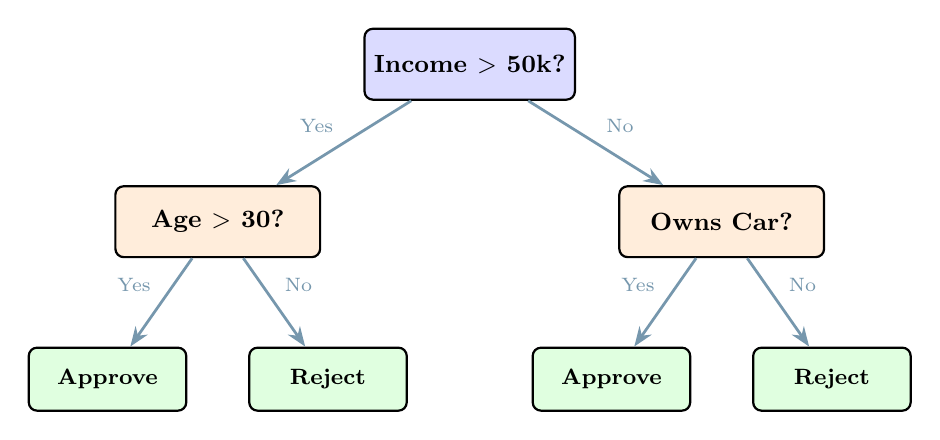
\begin{tikzpicture}[
  nd/.style={rectangle, draw, thick, fill=#1, minimum width=2.6cm, minimum height=0.9cm, align=center, font=\small\bfseries, rounded corners=3pt},
  lf/.style={rectangle, draw, thick, fill=green!12, minimum width=2.0cm, minimum height=0.8cm, align=center, font=\footnotesize\bfseries, rounded corners=3pt},
  arr/.style={-{Stealth[length=2.5mm]}, thick, primary!60, line width=1pt}
]
  \node[nd=blue!14]   (root) at (0,0)     {Income $>$ 50k?};
  \node[nd=orange!14] (n1)   at (-3.2,-2.0) {Age $>$ 30?};
  \node[nd=orange!14] (n2)   at (3.2,-2.0)  {Owns Car?};
  \node[lf]           (l1)   at (-4.6,-4.0) {Approve};
  \node[lf]           (l2)   at (-1.8,-4.0) {Reject};
  \node[lf]           (l3)   at (1.8,-4.0)  {Approve};
  \node[lf]           (l4)   at (4.6,-4.0)  {Reject};
  \draw[arr] (root) -- node[above left, font=\scriptsize]{Yes} (n1);
  \draw[arr] (root) -- node[above right, font=\scriptsize]{No} (n2);
  \draw[arr] (n1) -- node[above left, font=\scriptsize]{Yes} (l1);
  \draw[arr] (n1) -- node[above right, font=\scriptsize]{No} (l2);
  \draw[arr] (n2) -- node[above left, font=\scriptsize]{Yes} (l3);
  \draw[arr] (n2) -- node[above right, font=\scriptsize]{No} (l4);
\end{tikzpicture}
\end{center}

\begin{conceptbox}[Choosing the Best Split]
At each node, the algorithm picks the feature/threshold that most reduces impurity, measured by \textbf{Entropy} or the \textbf{Gini Index}:
$$
\text{Entropy}(S) = -\sum_{i} p_i \log_2 p_i, \qquad \text{Gini}(S) = 1 - \sum_i p_i^2
$$
\textbf{Information Gain} = Entropy(parent) $-$ weighted-average Entropy(children).
\end{conceptbox}

\begin{itemize}[leftmargin=*]
  \item \textbf{Pruning:} Limiting tree depth or removing branches to reduce overfitting.
  \item \textbf{Advantage:} Easy to interpret and visualize; handles both numeric and categorical features.
\end{itemize}

\subsection{Support Vector Machines (SVM)}
\begin{definitionbox}[Support Vector Machine]
An SVM finds the hyperplane that separates two classes with the \textbf{maximum margin} --- the largest possible distance to the nearest points of each class (the ``support vectors'').
\end{definitionbox}
\begin{itemize}[leftmargin=*]
  \item \textbf{Kernel Trick:} Maps data into a higher-dimensional space (e.g., via a polynomial or RBF kernel) so that classes that are not linearly separable in the original space become separable.
  \item \textbf{Soft Margin:} A tunable penalty ($C$) allows some misclassified points, trading margin width for fewer errors.
\end{itemize}

\begin{conceptbox}[Comparing the Classification Algorithms Covered So Far]
\rowcolors{2}{white}{lightbg}
\begin{center}
\begin{tabular}{@{}p{2.4cm}p{4.6cm}p{4.9cm}@{}}
\toprule
\rowcolor{secondary!25}
\textbf{Algorithm} & \textbf{Strength} & \textbf{Weakness} \\
\midrule
KNN & Simple, no training phase & Slow at prediction time, sensitive to scale \\
Naive Bayes & Fast, works well with text/high dimensions & Independence assumption rarely holds exactly \\
Decision Tree & Easy to interpret and visualize & Prone to overfitting if unpruned \\
SVM & Effective in high-dimensional spaces & Slower to train on very large datasets \\
\bottomrule
\end{tabular}
\end{center}
\end{conceptbox}

%=============================================================
\section{Ensemble Learning}
%=============================================================

\begin{definitionbox}[Ensemble Learning]
Ensemble learning combines predictions from multiple models to produce a result that is typically more accurate and robust than any single model alone.
\end{definitionbox}

\subsection{Bagging and Random Forests}
\begin{center}
\begin{tikzpicture}[
  nd/.style={rectangle, draw, thick, fill=#1, minimum width=2.4cm, minimum height=0.9cm, align=center, font=\footnotesize\bfseries, rounded corners=4pt,
    blur shadow={shadow blur steps=5, shadow xshift=0.5mm, shadow yshift=-0.5mm}},
  arr/.style={-{Stealth[length=2.5mm]}, thick, primary!60, line width=1pt}
]
  \node[nd=blue!12]   (data) at (2.6,1.6)  {\faIcon{database}~Training Data};
  \node[nd=orange!12] (t1)   at (0,0)      {Tree 1};
  \node[nd=orange!12] (t2)   at (2.6,0)    {Tree 2};
  \node[nd=orange!12] (t3)   at (5.2,0)    {Tree $N$};
  \node[nd=green!12]  (vote) at (2.6,-1.8) {\faIcon{check-circle}~Majority Vote / Average};
  \draw[arr] (data) -- (t1);
  \draw[arr] (data) -- (t2);
  \draw[arr] (data) -- (t3);
  \draw[arr] (t1) -- (vote);
  \draw[arr] (t2) -- (vote);
  \draw[arr] (t3) -- (vote);
\end{tikzpicture}
\end{center}

\begin{itemize}[leftmargin=*]
  \item \textbf{Bagging (Bootstrap Aggregating):} Trains many models on different random samples (with replacement) of the data, then averages/votes their predictions to reduce variance.
  \item \textbf{Random Forest:} Bagging applied to decision trees, with each tree also using a random subset of features at each split --- reduces correlation between trees.
\end{itemize}

\subsection{Boosting}
\begin{conceptbox}[How Boosting Works]
Boosting trains models \textbf{sequentially}, where each new model focuses on correcting the errors of the previous ones (e.g., by up-weighting misclassified samples), then combines them into a strong final predictor.
\end{conceptbox}
\begin{itemize}[leftmargin=*]
  \item \textbf{AdaBoost:} Re-weights misclassified training examples so subsequent weak learners focus on the hardest cases.
  \item \textbf{Gradient Boosting:} Each new model is trained to predict the \textit{residual error} of the ensemble so far (e.g., XGBoost, LightGBM).
\end{itemize}

\rowcolors{2}{white}{defbg}
\begin{center}
\begin{tabular}{@{}p{2.6cm}p{5.2cm}p{5.2cm}@{}}
\toprule
\rowcolor{primary!15}
\textbf{Aspect} & \textbf{Bagging} & \textbf{Boosting} \\
\midrule
Training Style & Parallel, independent models & Sequential, each model corrects prior errors \\
Goal & Reduce variance & Reduce bias \\
Overfitting Risk & Lower & Higher if not tuned carefully \\
Example & Random Forest & AdaBoost, XGBoost, LightGBM \\
\bottomrule
\end{tabular}
\end{center}

%=============================================================
\section{Unsupervised Learning: Clustering and Dimensionality Reduction}
%=============================================================

\begin{definitionbox}[Clustering]
Clustering groups data points so that points in the same group (cluster) are more similar to each other than to points in other groups, with no predefined labels.
\end{definitionbox}

\subsection{K-Means Clustering}
\begin{conceptbox}[The K-Means Algorithm]
\begin{enumerate}[leftmargin=*]
  \item Choose $k$ (the number of clusters) and randomly initialize $k$ centroids.
  \item \textbf{Assign:} Assign each point to its nearest centroid.
  \item \textbf{Update:} Recompute each centroid as the mean of the points assigned to it.
  \item Repeat Assign/Update until centroids stop changing (convergence).
\end{enumerate}
\end{conceptbox}
\begin{itemize}[leftmargin=*]
  \item \textbf{Choosing $k$:} The \textbf{Elbow Method} plots within-cluster variance against $k$ and looks for the ``elbow'' where improvement slows.
  \item \textbf{Limitation:} Assumes roughly spherical, similarly-sized clusters; sensitive to centroid initialization.
\end{itemize}

\subsection{Hierarchical Clustering}
\begin{itemize}[leftmargin=*]
  \item \textbf{Agglomerative (bottom-up):} Starts with every point as its own cluster, then repeatedly merges the two closest clusters.
  \item \textbf{Dendrogram:} A tree diagram showing the order and distance at which clusters were merged; cutting it at a chosen height yields a specific number of clusters.
\end{itemize}

\subsection{DBSCAN}
\begin{definitionbox}[DBSCAN]
Density-Based Spatial Clustering (DBSCAN) groups points that are closely packed together (dense regions), marking points in low-density regions as \textbf{noise/outliers}, and --- unlike K-Means --- does not require specifying the number of clusters in advance.
\end{definitionbox}

\subsection{Principal Component Analysis (PCA)}
\begin{definitionbox}[PCA]
PCA is a dimensionality reduction technique that projects data onto a smaller number of new axes (\textbf{principal components}) that capture the maximum possible variance in the data.
\end{definitionbox}

\begin{center}
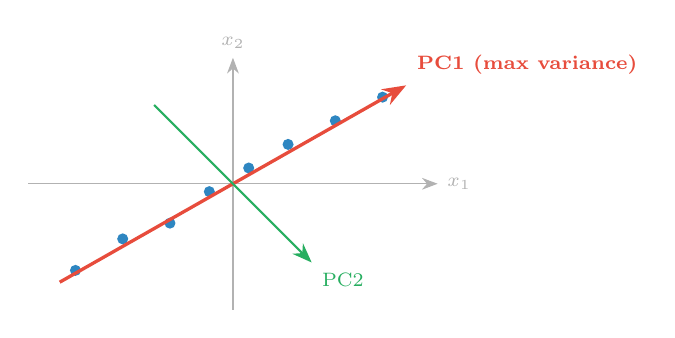
\begin{tikzpicture}[scale=1]
  \draw[-{Stealth[length=2mm]}, gray!60] (-2.6,0) -- (2.6,0) node[right, font=\scriptsize]{$x_1$};
  \draw[-{Stealth[length=2mm]}, gray!60] (0,-1.6) -- (0,1.6) node[above, font=\scriptsize]{$x_2$};
  \foreach \pt in {(-2,-1.1),(-1.4,-0.7),(-0.8,-0.5),(-0.3,-0.1),(0.2,0.2),(0.7,0.5),(1.3,0.8),(1.9,1.1)}{
    \fill[secondary] \pt circle (2pt);
  }
  \draw[-{Stealth[length=3mm]}, very thick, accent] (-2.2,-1.25) -- (2.2,1.25) node[above right, font=\scriptsize\bfseries]{PC1 (max variance)};
  \draw[-{Stealth[length=2.5mm]}, thick, greenhl] (-1.0,1.0) -- (1.0,-1.0) node[below right, font=\scriptsize]{PC2};
\end{tikzpicture}
\end{center}

\begin{itemize}[leftmargin=*]
  \item \textbf{Principal Components:} Orthogonal directions ranked by how much variance of the data they explain, derived from the eigenvectors of the data's covariance matrix.
  \item \textbf{Why Reduce Dimensions:} Speeds up training, reduces storage, fights the curse of dimensionality, and enables 2D/3D visualization of high-dimensional data.
  \item \textbf{Trade-off:} Some information (variance) is inevitably lost when discarding lower-ranked components.
\end{itemize}

%=============================================================
\section{Model Evaluation and Validation}
%=============================================================

\begin{definitionbox}[Why Evaluate?]
Model evaluation estimates how well a trained model will perform on new, unseen data --- the entire point of building a model in the first place.
\end{definitionbox}

\subsection{Train/Validation/Test Splits and Cross-Validation}
\begin{itemize}[leftmargin=*]
  \item \textbf{Training Set:} Used to fit the model's parameters.
  \item \textbf{Validation Set:} Used to tune hyperparameters and select between models.
  \item \textbf{Test Set:} Used only once, at the very end, to report final, unbiased performance.
  \item \textbf{k-Fold Cross-Validation:} Splits data into $k$ folds, trains on $k-1$ folds and validates on the remaining fold, rotating $k$ times and averaging the results --- more robust than a single split.
  \item \textbf{Stratified k-Fold:} Ensures each fold preserves the overall class proportions, important for imbalanced classification datasets.
  \item \textbf{Leave-One-Out Cross-Validation (LOOCV):} The extreme case of $k$-fold where $k$ equals the number of samples; thorough but computationally expensive.
\end{itemize}

\subsection{Classification Metrics}
\begin{center}
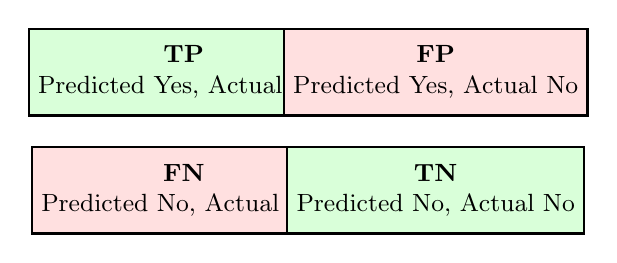
\begin{tikzpicture}[
  cell/.style={rectangle, draw, thick, minimum width=3.0cm, minimum height=1.1cm, align=center, font=\small},
]
  \node[cell, fill=green!15] (tp) at (0,0)     {\textbf{TP}\\Predicted Yes, Actual Yes};
  \node[cell, fill=red!12]   (fp) at (3.2,0)   {\textbf{FP}\\Predicted Yes, Actual No};
  \node[cell, fill=red!12]   (fn) at (0,-1.5)  {\textbf{FN}\\Predicted No, Actual Yes};
  \node[cell, fill=green!15] (tn) at (3.2,-1.5) {\textbf{TN}\\Predicted No, Actual No};
\end{tikzpicture}
\end{center}
$$
\text{Accuracy} = \frac{TP+TN}{TP+TN+FP+FN}, \qquad \text{Precision} = \frac{TP}{TP+FP}
$$
$$
\text{Recall} = \frac{TP}{TP+FN}, \qquad F_1 = \frac{2 \times \text{Precision} \times \text{Recall}}{\text{Precision} + \text{Recall}}
$$
\begin{conceptbox}[When Accuracy Is Misleading]
On an imbalanced dataset (e.g., 95\% non-fraud, 5\% fraud), a model that always predicts ``non-fraud'' scores 95\% accuracy while catching zero fraud --- Precision, Recall, and $F_1$ reveal this failure; \textbf{ROC-AUC} summarizes performance across all classification thresholds.
\end{conceptbox}

\subsection{Regression Metrics}
$$
MAE = \frac{1}{m}\sum_{i=1}^{m}\left|y^{(i)}-\hat{y}^{(i)}\right|, \qquad
MSE = \frac{1}{m}\sum_{i=1}^{m}\left(y^{(i)}-\hat{y}^{(i)}\right)^2
$$
$$
RMSE = \sqrt{MSE}, \qquad R^2 = 1 - \frac{\sum_i (y^{(i)}-\hat{y}^{(i)})^2}{\sum_i (y^{(i)}-\bar{y})^2}
$$
\begin{itemize}[leftmargin=*]
  \item $R^2$ (coefficient of determination) close to 1 means the model explains most of the variance in the target; close to 0 means it explains almost none.
\end{itemize}

%=============================================================
\section{Overfitting, Underfitting, and Regularization}
%=============================================================

\begin{definitionbox}[Overfitting and Underfitting]
Overfitting occurs when a model learns the training data too well, including its noise, and fails to generalize; underfitting occurs when a model is too simple to capture the underlying pattern at all.
\end{definitionbox}

\subsection{The Bias-Variance Tradeoff}
\rowcolors{2}{white}{defbg}
\begin{center}
\begin{tabular}{@{}p{2.6cm}p{5.2cm}p{5.2cm}@{}}
\toprule
\rowcolor{primary!15}
\textbf{Aspect} & \textbf{High Bias (Underfitting)} & \textbf{High Variance (Overfitting)} \\
\midrule
Training Error & High & Low \\
Test Error & High & High \\
Model Complexity & Too simple & Too complex \\
Fix & Add features, more complex model & More data, regularization, simplify model \\
\bottomrule
\end{tabular}
\end{center}

\subsection{L1/L2 Regularization}
\begin{conceptbox}[Penalizing Complexity]
Regularization adds a penalty term to the cost function to discourage overly large weights, trading a little training accuracy for better generalization:
$$
J_{\text{L2}}(w) = J(w) + \lambda \sum_j w_j^2 \qquad \text{(Ridge)}
$$
$$
J_{\text{L1}}(w) = J(w) + \lambda \sum_j |w_j| \qquad \text{(Lasso)}
$$
L1 (Lasso) can shrink some weights to exactly zero, performing automatic feature selection; L2 (Ridge) shrinks weights smoothly without eliminating them.
\end{conceptbox}

\subsection{Hyperparameter Tuning}
\begin{itemize}[leftmargin=*]
  \item \textbf{Hyperparameter:} A setting chosen before training (e.g., $k$ in KNN, tree depth, learning rate $\alpha$, regularization strength $\lambda$) --- not learned from data directly.
  \item \textbf{Grid Search:} Exhaustively tries all combinations from a predefined set of hyperparameter values.
  \item \textbf{Random Search:} Samples random combinations, often finding good settings faster than grid search for large search spaces.
\end{itemize}

%=============================================================
\section{Introduction to Neural Networks}
%=============================================================

\begin{definitionbox}[Artificial Neural Network]
An artificial neural network is a model loosely inspired by biological neurons, composed of layers of simple computing units (neurons) connected by weighted links that are adjusted during training.
\end{definitionbox}

\subsection{The Perceptron and Multi-Layer Perceptron}
\begin{center}
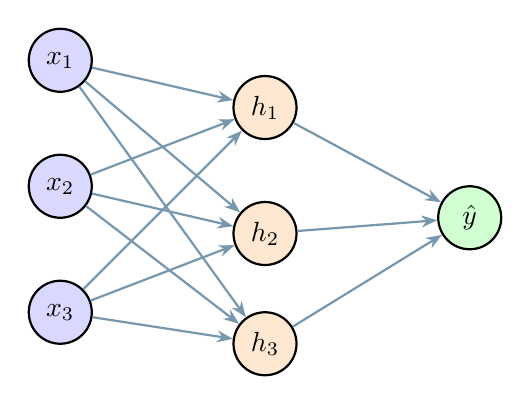
\begin{tikzpicture}[
  neuron/.style={circle, draw, thick, fill=#1, minimum size=0.8cm},
  arr/.style={-{Stealth[length=2mm]}, primary!60, line width=0.8pt}
]
  \node[neuron=blue!15] (i1) at (0,1.6)  {$x_1$};
  \node[neuron=blue!15] (i2) at (0,0)    {$x_2$};
  \node[neuron=blue!15] (i3) at (0,-1.6) {$x_3$};
  \node[neuron=orange!18] (h1) at (2.6,1.0) {$h_1$};
  \node[neuron=orange!18] (h2) at (2.6,-0.6) {$h_2$};
  \node[neuron=orange!18] (h3) at (2.6,-2.0) {$h_3$};
  \node[neuron=green!18] (o1) at (5.2,-0.4) {$\hat{y}$};
  \foreach \i in {i1,i2,i3}{
    \foreach \h in {h1,h2,h3}{
      \draw[arr] (\i) -- (\h);
    }
  }
  \foreach \h in {h1,h2,h3}{
    \draw[arr] (\h) -- (o1);
  }
\end{tikzpicture}
\end{center}

\begin{itemize}[leftmargin=*]
  \item \textbf{Perceptron:} A single neuron computes a weighted sum of inputs plus a bias, then applies an activation function: $\hat{y} = f\left(\sum_i w_i x_i + b\right)$.
  \item \textbf{Multi-Layer Perceptron (MLP):} Stacks an input layer, one or more \textbf{hidden layers}, and an output layer, allowing the network to model non-linear relationships.
\end{itemize}

\subsection{Activation Functions}
\rowcolors{2}{white}{defbg}
\begin{center}
\begin{tabular}{@{}p{2.2cm}p{5.6cm}p{5.2cm}@{}}
\toprule
\rowcolor{primary!15}
\textbf{Function} & \textbf{Formula} & \textbf{Typical Use} \\
\midrule
Sigmoid & $\sigma(z) = \frac{1}{1+e^{-z}}$ & Binary classification output layer \\
ReLU & $f(z) = \max(0,z)$ & Hidden layers (fast, avoids vanishing gradient) \\
Softmax & $\frac{e^{z_i}}{\sum_j e^{z_j}}$ & Multi-class classification output layer \\
\bottomrule
\end{tabular}
\end{center}

\subsection{Backpropagation}
\begin{conceptbox}[How Networks Learn]
Backpropagation computes how much each weight contributed to the final error by applying the chain rule of calculus backward through the network, then gradient descent updates every weight to reduce that error.
\end{conceptbox}

%=============================================================
\section{Introduction to Deep Learning}
%=============================================================

\begin{definitionbox}[Deep Learning]
Deep learning uses neural networks with many hidden layers (``deep'' architectures) to automatically learn hierarchical feature representations directly from raw data such as pixels or text.
\end{definitionbox}

\subsection{Convolutional Neural Networks (CNNs)}
\begin{conceptbox}[How CNNs Process Images]
\begin{itemize}[leftmargin=*]
  \item \textbf{Convolution Layer:} Slides small filters (kernels) across the image to detect local patterns (edges, textures).
  \item \textbf{Pooling Layer:} Downsamples feature maps (e.g., max pooling) to reduce size and add translation invariance.
  \item \textbf{Fully Connected Layer:} Combines the extracted features to make the final classification.
\end{itemize}
CNNs dominate computer vision tasks: image classification, object detection, facial recognition.
\end{conceptbox}

\subsection{Recurrent Neural Networks (RNNs)}
\begin{definitionbox}[Recurrent Neural Network]
An RNN processes sequential data (text, time series, audio) by maintaining a hidden state that is updated at each time step, allowing information from earlier steps to influence later predictions.
\end{definitionbox}
\begin{itemize}[leftmargin=*]
  \item \textbf{Vanishing Gradient Problem:} Standard RNNs struggle to learn long-range dependencies because gradients shrink as they propagate back through many time steps.
  \item \textbf{LSTM/GRU:} Gated variants of RNNs designed to retain relevant information over longer sequences.
  \item \textbf{Transfer Learning:} Reusing a large model pretrained on a general dataset and fine-tuning it on a smaller, task-specific dataset, saving time and data compared to training from scratch.
\end{itemize}

%=============================================================
\section{Reinforcement Learning Basics}
%=============================================================

\begin{definitionbox}[Reinforcement Learning]
Reinforcement Learning (RL) is a learning paradigm in which an \textbf{agent} learns to make decisions by taking \textbf{actions} in an \textbf{environment} to maximize cumulative \textbf{reward}.
\end{definitionbox}

\subsection{Agents, Environments, and Rewards}
\begin{center}
\begin{tikzpicture}[
  box/.style={rectangle, draw, thick, fill=#1, minimum width=3.2cm, minimum height=1.3cm, align=center, font=\small\bfseries, rounded corners=4pt,
    blur shadow={shadow blur steps=5, shadow xshift=0.5mm, shadow yshift=-0.5mm}},
  arr/.style={-{Stealth[length=2.5mm]}, very thick, primary!60, line width=1.2pt}
]
  \node[box=blue!14]   (agent) at (0,0)   {\faIcon{robot}~Agent};
  \node[box=orange!14] (env)   at (6,0)   {\faIcon{globe}~Environment};
  \draw[arr] (agent.north east) to[bend left=30] node[above, font=\scriptsize]{Action $a_t$} (env.north west);
  \draw[arr] (env.south west) to[bend left=30] node[below, font=\scriptsize]{State $s_{t+1}$, Reward $r_{t+1}$} (agent.south east);
\end{tikzpicture}
\end{center}

\begin{itemize}[leftmargin=*]
  \item \textbf{Policy ($\pi$):} The agent's strategy mapping states to actions.
  \item \textbf{Reward Signal:} Immediate feedback (positive or negative) after an action.
  \item \textbf{Episode:} One complete run from a start state to a terminal state (e.g., one game).
  \item \textbf{Exploration vs.\ Exploitation:} The agent must balance trying new actions (exploration) against using known good actions (exploitation).
\end{itemize}

\subsection{Q-Learning}
\begin{definitionbox}[Q-Learning]
Q-Learning learns a table of action-values $Q(s,a)$ estimating the expected future reward of taking action $a$ in state $s$, updated after every step using the Bellman equation.
\end{definitionbox}
$$
Q(s,a) \leftarrow Q(s,a) + \alpha\Big[r + \gamma \max_{a'} Q(s',a') - Q(s,a)\Big]
$$
\begin{itemize}[leftmargin=*]
  \item $\alpha$ (learning rate) controls how much new information overrides old estimates.
  \item $\gamma$ (discount factor, $0 \leq \gamma \leq 1$) controls how much future rewards matter relative to immediate ones.
\end{itemize}

%=============================================================
\section{The Machine Learning Pipeline and Deployment}
%=============================================================

\begin{definitionbox}[ML Pipeline]
An ML pipeline is the automated sequence of steps --- data ingestion, preprocessing, training, evaluation, and deployment --- that turns raw data into a model serving real predictions in production.
\end{definitionbox}

\subsection{From Notebook to Production}
\begin{itemize}[leftmargin=*]
  \item \textbf{Experimentation:} Data scientists prototype models in notebooks (Jupyter) on a static dataset.
  \item \textbf{Productionization:} The winning model is wrapped in an API (e.g., a REST endpoint) so other applications can request predictions.
  \item \textbf{Batch vs.\ Real-Time Inference:} Batch scores many records periodically (e.g., nightly); real-time inference responds to individual requests within milliseconds.
\end{itemize}

\subsection{Model Monitoring and Drift}
\begin{conceptbox}[Why Deployed Models Need Monitoring]
\begin{itemize}[leftmargin=*]
  \item \textbf{Data Drift:} The statistical properties of incoming data change over time relative to the training data.
  \item \textbf{Concept Drift:} The relationship between inputs and the correct output changes over time (e.g., customer behavior shifts).
  \item \textbf{Model Retraining:} Deployed models are periodically retrained on fresh data to stay accurate as drift accumulates.
\end{itemize}
\end{conceptbox}

%=============================================================
\section{Ethical and Responsible Machine Learning}
%=============================================================

\begin{definitionbox}[Why Ethics Matters in ML]
Because ML models are trained on real-world data, they can inherit and amplify the biases present in that data, making responsible design and evaluation essential before deployment.
\end{definitionbox}

\begin{alertbox}[Key Concerns]
\begin{itemize}[leftmargin=*]
  \item \textbf{Bias and Fairness:} A model trained on biased historical data (e.g., biased hiring decisions) can learn and perpetuate that bias.
  \item \textbf{Explainability:} Complex models (deep neural networks, large ensembles) can be ``black boxes,'' making decisions hard to justify, especially in high-stakes domains (credit, healthcare, criminal justice).
  \item \textbf{Privacy:} Training data may contain sensitive personal information that must be protected and anonymized.
  \item \textbf{Accountability:} It must be clear who is responsible when an ML system makes a harmful or incorrect decision.
  \item \textbf{Robustness:} Models can be fooled by adversarial examples --- inputs deliberately perturbed to cause misclassification.
\end{itemize}
\end{alertbox}

\begin{conceptbox}[Building Responsible ML Systems]
\begin{itemize}[leftmargin=*]
  \item Audit training data and model outputs for disparate impact across demographic groups.
  \item Use interpretable models or explainability tools (e.g., feature importance, SHAP values) where decisions must be justified.
  \item Keep a human in the loop for high-stakes decisions rather than fully automating them.
  \item Document data sources, model assumptions, and limitations (``model cards'').
\end{itemize}
\end{conceptbox}

%=============================================================
\section{Core Mathematical Foundations for Machine Learning}
%=============================================================

\begin{definitionbox}[Why Math Matters for ML]
Linear algebra, probability, and calculus are the mathematical languages used to represent data, quantify uncertainty, and optimize model parameters in every ML algorithm.
\end{definitionbox}

\subsection{Linear Algebra Essentials}
\begin{itemize}[leftmargin=*]
  \item \textbf{Vector:} An ordered list of numbers representing a data point or a set of weights.
  \item \textbf{Matrix:} A 2D array of numbers, e.g., an entire dataset (rows = samples, columns = features).
  \item \textbf{Dot Product:} $\mathbf{a}\cdot\mathbf{b} = \sum_i a_i b_i$, the core operation behind a neuron's weighted sum.
  \item \textbf{Eigenvectors/Eigenvalues:} Special directions/scales used by PCA to find directions of maximum variance.
\end{itemize}

\subsection{Probability and Statistics Essentials}
\begin{itemize}[leftmargin=*]
  \item \textbf{Conditional Probability:} $P(A\mid B) = \dfrac{P(A \cap B)}{P(B)}$, the basis of Bayes' Theorem and Naive Bayes.
  \item \textbf{Mean and Variance:} Measure the center and spread of a feature's distribution; used in standardization.
  \item \textbf{Bayes' Theorem:} $P(A\mid B) = \dfrac{P(B\mid A)\,P(A)}{P(B)}$.
\end{itemize}

\subsection{Calculus and Optimization Essentials}
\begin{itemize}[leftmargin=*]
  \item \textbf{Derivative:} Measures the rate of change of a function; the gradient generalizes this to multiple variables.
  \item \textbf{Gradient:} A vector of partial derivatives pointing in the direction of steepest increase of a function --- gradient descent moves in the \textit{opposite} direction to minimize cost.
  \item \textbf{Convex Function:} A function with a single global minimum (like MSE for linear regression), making optimization reliable.
\end{itemize}

%=============================================================
\section{Exam-Oriented Worked Examples}
%=============================================================

\begin{examplebox}[Worked Example 1: Linear Regression Prediction]
A fitted model is $\hat{y} = 5 + 2x$. Predict $\hat{y}$ for $x=7$:
$$
\hat{y} = 5 + 2(7) = 19
$$
\end{examplebox}

\begin{examplebox}[Worked Example 2: One Gradient Descent Step]
Given $w=4$, gradient $\frac{\partial J}{\partial w}=6$, and learning rate $\alpha=0.1$:
$$
w := 4 - 0.1(6) = 4 - 0.6 = 3.4
$$
\end{examplebox}

\begin{examplebox}[Worked Example 3: KNN Classification ($k=3$)]
A new point's 3 nearest neighbors have labels \{Cat, Cat, Dog\}. By majority vote, the new point is classified as \textbf{Cat} (2 out of 3 votes).
\end{examplebox}

\begin{examplebox}[Worked Example 4: Entropy and Information Gain]
A node has 10 examples: 6 positive, 4 negative:
$$
\text{Entropy} = -\frac{6}{10}\log_2\frac{6}{10} - \frac{4}{10}\log_2\frac{4}{10} \approx 0.971
$$
A pure split (all-positive / all-negative children) would give Information Gain $\approx 0.971$, the maximum possible for this node.
\end{examplebox}

\begin{examplebox}[Worked Example 5: Confusion Matrix Metrics]
Given $TP=40$, $FP=10$, $FN=5$, $TN=45$:
$$
\text{Precision} = \frac{40}{40+10} = 0.80, \qquad \text{Recall} = \frac{40}{40+5} \approx 0.889
$$
$$
F_1 = \frac{2(0.80)(0.889)}{0.80+0.889} \approx 0.842
$$
\end{examplebox}

\begin{examplebox}[Worked Example 6: One K-Means Update]
Cluster points $(2,2)$, $(4,4)$, and $(6,4)$ are assigned to the same centroid. The new centroid is their mean:
$$
\left(\frac{2+4+6}{3}, \frac{2+4+4}{3}\right) = (4, 3.33)
$$
\end{examplebox}

\begin{examplebox}[Worked Example 7: Naive Bayes Classification]
Classify a message with word ``win'' as spam/ham given $P(\text{spam})=0.3$, $P(\text{``win''}\mid\text{spam})=0.8$, $P(\text{ham})=0.7$, $P(\text{``win''}\mid\text{ham})=0.05$:
$$
P(\text{spam})\times P(\text{``win''}\mid\text{spam}) = 0.3 \times 0.8 = 0.24
$$
$$
P(\text{ham})\times P(\text{``win''}\mid\text{ham}) = 0.7 \times 0.05 = 0.035
$$
Since $0.24 > 0.035$, classify as \textbf{spam}.
\end{examplebox}

\begin{examplebox}[Worked Example 8: Regression Error Metrics]
Actual values $y = [3, 5, 2]$, predictions $\hat{y} = [2, 5, 4]$:
$$
MAE = \frac{|3-2|+|5-5|+|2-4|}{3} = \frac{1+0+2}{3} = 1.0
$$
$$
MSE = \frac{1^2+0^2+2^2}{3} = \frac{5}{3} \approx 1.67, \qquad RMSE \approx 1.29
$$
\end{examplebox}

%=============================================================
\section{Quick Revision Glossary}
%=============================================================

\rowcolors{2}{white}{defbg}
\begin{longtable}{@{}p{3.3cm}p{10.2cm}@{}}
\toprule
\rowcolor{primary!15}
\textbf{Term} & \textbf{One-Line Meaning} \\
\midrule
\endhead
Machine Learning & Field enabling computers to learn patterns from data instead of fixed rules. \\
\addlinespace
Supervised Learning & Learning a mapping from labeled input-output pairs. \\
\addlinespace
Unsupervised Learning & Finding structure in unlabeled data. \\
\addlinespace
Reinforcement Learning & Learning a policy via rewards from interacting with an environment. \\
\addlinespace
Feature & A measurable input property used by a model. \\
\addlinespace
Label & The known, correct output for a training example in supervised learning. \\
\addlinespace
Feature Engineering & Creating new, more informative features from raw data. \\
\addlinespace
Curse of Dimensionality & Data becomes sparse and harder to learn from as feature count grows. \\
\addlinespace
Overfitting & Model fits training noise and fails to generalize to new data. \\
\addlinespace
Underfitting & Model is too simple to capture the underlying pattern. \\
\addlinespace
Bias-Variance Tradeoff & Balancing model simplicity (bias) against sensitivity to training data (variance). \\
\addlinespace
Regularization & Penalty added to the cost function to discourage overly complex models. \\
\addlinespace
Linear Regression & Predicts a continuous value as a weighted linear combination of features. \\
\addlinespace
Logistic Regression & Predicts class probability via the sigmoid of a linear combination of features. \\
\addlinespace
Gradient Descent & Iterative optimization that updates weights opposite to the cost gradient. \\
\addlinespace
K-Nearest Neighbors (KNN) & Classifies a point by majority vote among its $k$ closest training points. \\
\addlinespace
Naive Bayes & Bayes'-Theorem-based classifier assuming conditional feature independence. \\
\addlinespace
Decision Tree & Splits data on feature thresholds to reach a label at each leaf. \\
\addlinespace
Entropy & Measure of impurity/disorder used to choose decision tree splits. \\
\addlinespace
Support Vector Machine (SVM) & Finds the maximum-margin hyperplane separating classes. \\
\addlinespace
Ensemble Learning & Combining multiple models' predictions for better accuracy/robustness. \\
\addlinespace
Bagging & Trains models in parallel on bootstrapped samples and averages/votes results. \\
\addlinespace
Random Forest & Bagged decision trees, each using a random subset of features per split. \\
\addlinespace
Boosting & Trains models sequentially, each correcting the previous ones' errors. \\
\addlinespace
K-Means Clustering & Iteratively assigns points to the nearest of $k$ centroids and updates them. \\
\addlinespace
Hierarchical Clustering & Builds a tree of clusters by repeatedly merging the closest pair. \\
\addlinespace
DBSCAN & Density-based clustering that also detects noise/outlier points. \\
\addlinespace
Principal Component Analysis (PCA) & Projects data onto directions of maximum variance to reduce dimensions. \\
\addlinespace
Cross-Validation & Rotating train/validation splits ($k$-fold) for a more robust performance estimate. \\
\addlinespace
Confusion Matrix & Table of TP/FP/FN/TN counts summarizing classification results. \\
\addlinespace
Precision & Of predicted positives, the fraction that are actually positive. \\
\addlinespace
Recall & Of actual positives, the fraction correctly predicted positive. \\
\addlinespace
F1 Score & Harmonic mean of precision and recall. \\
\addlinespace
ROC-AUC & Area under the ROC curve; summarizes performance across all thresholds. \\
\addlinespace
RMSE & Root Mean Squared Error; regression error metric in the same units as the target. \\
\addlinespace
Hyperparameter & A model setting chosen before training rather than learned from data. \\
\addlinespace
Neural Network & Layers of connected neurons that learn weighted transformations of input data. \\
\addlinespace
Activation Function & Non-linear function applied at each neuron (e.g., ReLU, Sigmoid, Softmax). \\
\addlinespace
Backpropagation & Chain-rule-based algorithm for computing gradients through a neural network. \\
\addlinespace
Convolutional Neural Network (CNN) & Deep network using convolution/pooling layers, dominant in computer vision. \\
\addlinespace
Recurrent Neural Network (RNN) & Neural network with a hidden state for processing sequential data. \\
\addlinespace
Q-Learning & Reinforcement learning method that learns action-values via the Bellman equation. \\
\addlinespace
Data Drift & Change over time in the statistical properties of incoming data. \\
\addlinespace
Model Card & Documentation of a model's data, assumptions, and limitations. \\
\addlinespace
Data Leakage & Information from outside the training set unintentionally influences training. \\
\addlinespace
One-Hot Encoding & Represents a categorical variable as binary indicator columns. \\
\addlinespace
Grid Search & Exhaustive search over a predefined set of hyperparameter combinations. \\
\addlinespace
Elbow Method & Plots within-cluster variance against $k$ to help choose the number of clusters. \\
\addlinespace
Exploration vs.\ Exploitation & The RL agent's tradeoff between trying new actions and using known good ones. \\
\addlinespace
Transfer Learning & Fine-tuning a model pretrained on a large general dataset for a new, specific task. \\
\addlinespace
Learning Rate & Step size $\alpha$ controlling how much weights change per gradient descent update. \\
\addlinespace
Stratified k-Fold & Cross-validation variant that preserves class proportions in each fold. \\
\bottomrule
\end{longtable}

%=============================================================
\section{Question Bank Blueprint (80 Marks Support)}
%=============================================================

\begin{conceptbox}[Suggested 80 Marks Distribution]
\begin{itemize}[leftmargin=*]
  \item \textbf{Section A:} MCQs and definitions (20 marks)
  \item \textbf{Section B:} Short conceptual questions (20 marks)
  \item \textbf{Section C:} Descriptive/theory questions (20 marks)
  \item \textbf{Section D:} Numerical/problem-solving questions (20 marks)
\end{itemize}
\end{conceptbox}

\subsection{Important Theory Questions}
\begin{itemize}[leftmargin=*]
  \item Differentiate supervised, unsupervised, and reinforcement learning with examples.
  \item Explain the complete machine learning workflow from data collection to deployment.
  \item Differentiate feature scaling techniques: min-max scaling versus standardization.
  \item Explain gradient descent and the effect of the learning rate on convergence.
  \item Differentiate linear regression and logistic regression.
  \item Explain how K-Nearest Neighbors classifies a new point, and the effect of choosing $k$.
  \item Explain how a decision tree chooses the best feature to split on.
  \item Differentiate bagging and boosting as ensemble techniques.
  \item Explain the K-Means clustering algorithm and how the number of clusters is chosen.
  \item Explain Principal Component Analysis and why dimensionality reduction is useful.
  \item Explain why accuracy can be a misleading metric, and how precision/recall address this.
  \item Explain the bias-variance tradeoff and how it relates to overfitting and underfitting.
  \item Differentiate L1 and L2 regularization.
  \item Explain backpropagation and its role in training neural networks.
  \item Differentiate CNNs and RNNs in terms of the type of data they are best suited for.
  \item Explain the agent-environment loop in reinforcement learning and the Q-Learning update rule.
  \item Discuss ethical concerns in machine learning such as bias, explainability, and privacy.
\end{itemize}

\subsection{Important Numerical/Analytical Questions}
\begin{itemize}[leftmargin=*]
  \item Predict an output value given a fitted linear regression equation.
  \item Compute one gradient descent update given a weight, gradient, and learning rate.
  \item Classify a point using KNN given its nearest neighbors' labels.
  \item Compute entropy and information gain for a given split of examples.
  \item Compute precision, recall, and F1 score from a confusion matrix.
  \item Compute the updated centroid after one K-Means assignment step.
  \item Classify a message using Naive Bayes given simple probability tables.
  \item Compute MAE, MSE, and RMSE given actual and predicted values.
\end{itemize}

\subsection{Sample MCQs with Answer Key}
\begin{enumerate}[leftmargin=*]
  \item Which learning paradigm uses labeled input-output pairs?\\
  (a) Unsupervised Learning \quad (b) Supervised Learning \quad (c) Reinforcement Learning \quad (d) Semi-Supervised Learning
  \item Which algorithm has no explicit training phase and classifies by distance to neighbors?\\
  (a) Decision Tree \quad (b) Naive Bayes \quad (c) K-Nearest Neighbors \quad (d) Logistic Regression
  \item Which metric measures impurity used to choose decision tree splits?\\
  (a) Entropy \quad (b) Precision \quad (c) RMSE \quad (d) Learning Rate
  \item Bagging primarily helps reduce which problem?\\
  (a) Bias \quad (b) Variance \quad (c) Learning rate \quad (d) Data drift
  \item Which algorithm does not require specifying the number of clusters in advance?\\
  (a) K-Means \quad (b) Hierarchical Clustering \quad (c) DBSCAN \quad (d) PCA
  \item Which metric is the harmonic mean of precision and recall?\\
  (a) Accuracy \quad (b) F1 Score \quad (c) RMSE \quad (d) $R^2$
  \item Which regularization technique can shrink some weights to exactly zero?\\
  (a) L1 (Lasso) \quad (b) L2 (Ridge) \quad (c) Dropout \quad (d) Batch Normalization
  \item Which neural network architecture is best suited to sequential data such as text or time series?\\
  (a) CNN \quad (b) RNN \quad (c) Random Forest \quad (d) SVM
  \item In Q-Learning, what does the discount factor $\gamma$ control?\\
  (a) Learning speed \quad (b) The weight given to future rewards \quad (c) The number of actions \quad (d) The exploration rate only
\end{enumerate}
\begin{conceptbox}[Answer Key]
1--(b), 2--(c), 3--(a), 4--(b), 5--(c), 6--(b), 7--(a), 8--(b), 9--(b)
\end{conceptbox}

%=============================================================
\section{Summary}
%=============================================================

\begin{examplebox}[Key Takeaways]
\begin{itemize}[leftmargin=*]
  \item Machine learning infers models directly from data, spanning supervised, unsupervised, and reinforcement learning paradigms.
  \item Careful data preprocessing and feature engineering underpin the performance of every downstream algorithm.
  \item Regression (linear/logistic), distance/probability-based methods (KNN, Naive Bayes), trees and margins (Decision Trees, SVM), and ensembles (bagging, boosting) form the core supervised toolkit.
  \item Clustering (K-Means, hierarchical, DBSCAN) and PCA reveal structure in unlabeled data and reduce dimensionality.
  \item Rigorous evaluation (cross-validation, confusion-matrix metrics, regression metrics) and awareness of the bias-variance tradeoff prevent overfitting/underfitting.
  \item Neural networks and deep learning (CNNs, RNNs) extend ML to images, text, and sequences via backpropagation.
  \item Reinforcement learning, production ML pipelines, and responsible/ethical practice complete the path from a trained model to a trustworthy, deployed system.
\end{itemize}
\end{examplebox}

\end{document}
